\documentclass{beeper}

\usepackage{fontawesome}
\usepackage{etoolbox}
\usepackage{textcomp}
\usepackage[nodisplayskipstretch]{setspace}
\usepackage{xspace}
\usepackage{verbatim}
\usepackage{multicol}
\usepackage{soul}
\usepackage{attrib}

\usepackage{amsmath,amssymb,amsthm}

\usepackage[linesnumbered,commentsnumbered,ruled,vlined]{algorithm2e}
\newcommand\mycommfont[1]{\footnotesize\ttfamily\textcolor{blue}{#1}}
\SetCommentSty{mycommfont}
\SetKwComment{tcc}{ \# }{}
\SetKwComment{tcp}{ \# }{}

\usepackage{siunitx}

\usepackage{tikz}
\usepackage{pgfplots}
\usetikzlibrary{decorations.pathreplacing,calc,arrows.meta,shapes,graphs}

\AtBeginEnvironment{minted}{\singlespacing\fontsize{10}{10}\selectfont}
\setmainfont{Open Sans Light}
\usefonttheme{serif}

\makeatletter
\patchcmd{\beamer@sectionintoc}{\vskip1.5em}{\vskip0.5em}{}{}
\makeatother

% Math stuffs
\newcommand{\Z}{\mathbb{Z}}
\newcommand{\R}{\mathbb{R}}
\newcommand{\N}{\mathbb{N}}
\newcommand{\lcm}{\text{lcm}}
\newcommand{\Inn}{\text{Inn}}
\newcommand{\Aut}{\text{Aut}}
\newcommand{\Ker}{\text{Ker}\ }
\newcommand{\la}{\langle}
\newcommand{\ra}{\rangle}

\newcommand{\yournewcommand}[2]{Something #1, and #2}

\newenvironment{question}[1]{\par\textbf{Question #1.}\par}{}

\newcommand{\pmidg}[1]{\parbox{\widthof{#1}}{#1}}
\newcommand{\splitslide}[4]{
    \noindent
    \begin{minipage}{#1 \textwidth - #2 }
        #3
    \end{minipage}%
    \hspace{ \dimexpr #2 * 2 \relax }%
    \begin{minipage}{\textwidth - #1 \textwidth - #2 }
        #4
    \end{minipage}
}

\newcommand{\frameoutput}[1]{\frame{\colorbox{white}{#1}}}

\newcommand{\tikzmark}[1]{%
\tikz[baseline=-0.55ex,overlay,remember picture] \node[inner sep=0pt,] (#1)
{\vphantom{T}};
}

\newcommand{\braced}[3]{%
    \begin{tikzpicture}[overlay,remember picture]
        \draw [thick,decorate,decoration={brace,raise=1ex,amplitude=4pt},blue] (#2.south west-|T1.south west) -- node[anchor=west,left,xshift=-1.8ex,text=olive]{#3} (#1.north west-|T1.south west);
    \end{tikzpicture}
}

\title{Hungryserv}
\subtitle{A Homeserver Optimized for Unfederated Use-Cases}
\author{Sumner Evans}
\institute{Beeper}
\date{26 August 2022}

\begin{document}

\begin{frame}{A bit about me}
    My name is Sumner, I'm a \textbf{software engineer at Beeper}.
    \begin{itemize}
        \item I graduated from Colorado School of Mines in 2019 with a master's
            in CS.
        \item I teach as an adjunct professor at my alma mater.
        \item I enjoy skiing, volleyball, and football (soccer).
        \item I'm a 4th degree black belt in ATA taekwondo.
    \end{itemize}
    \pause

    I became interested in Matrix when I was the chair of the ACM chapter at
    Mines. I was looking for an open source chat platform for the club to use,
    and Matrix fit the bill!
\end{frame}

\begin{frame}{What I work on at Beeper}
    I am on the newly created \textit{Scaling} team.

    Our current objective is to prepare Beeper for rocket-ship growth.
    \pause

    I was previously part of the \textit{Bridges} team. 

    Notable projects include:
    \begin{itemize}
        \item Writing the LinkedIn bridge
        \item Implementing massive stability improvements in the Signal bridge
        \item Implementing incremental infinite backfill in our WhatsApp and
            Facebook bridges
    \end{itemize}
\end{frame}

\begin{frame}{Overview}
    \setbeamertemplate{section in toc}[sections numbered]
    \tableofcontents[hideallsubsections]

    \begin{block}{This talk is interactive!}
        If you have questions at any point, feel free to interrupt me.
    \end{block}
\end{frame}

\section{A bit about Beeper}

\begin{frame}{Beeper's mission}
    Our mission is to:\\

    \begin{quote}
        make it easy for everyone on Earth to chat with each other.
    \end{quote}
    \pause

    We specifically chose the word ``chat'' rather than ``communicate'' because
    we are focusing on \textit{people talking to one another}.
\end{frame}

\begin{frame}{How we are getting there}
    % focusing on DMs not group chats
    % bring all your chats to the same place - switch with no cost

    % We encourage users to connect \textbf{all} of their chat networks.
\end{frame}

\section{A bit about Beeper's current architecture}

\begin{frame}{A diagram}
    \centerline{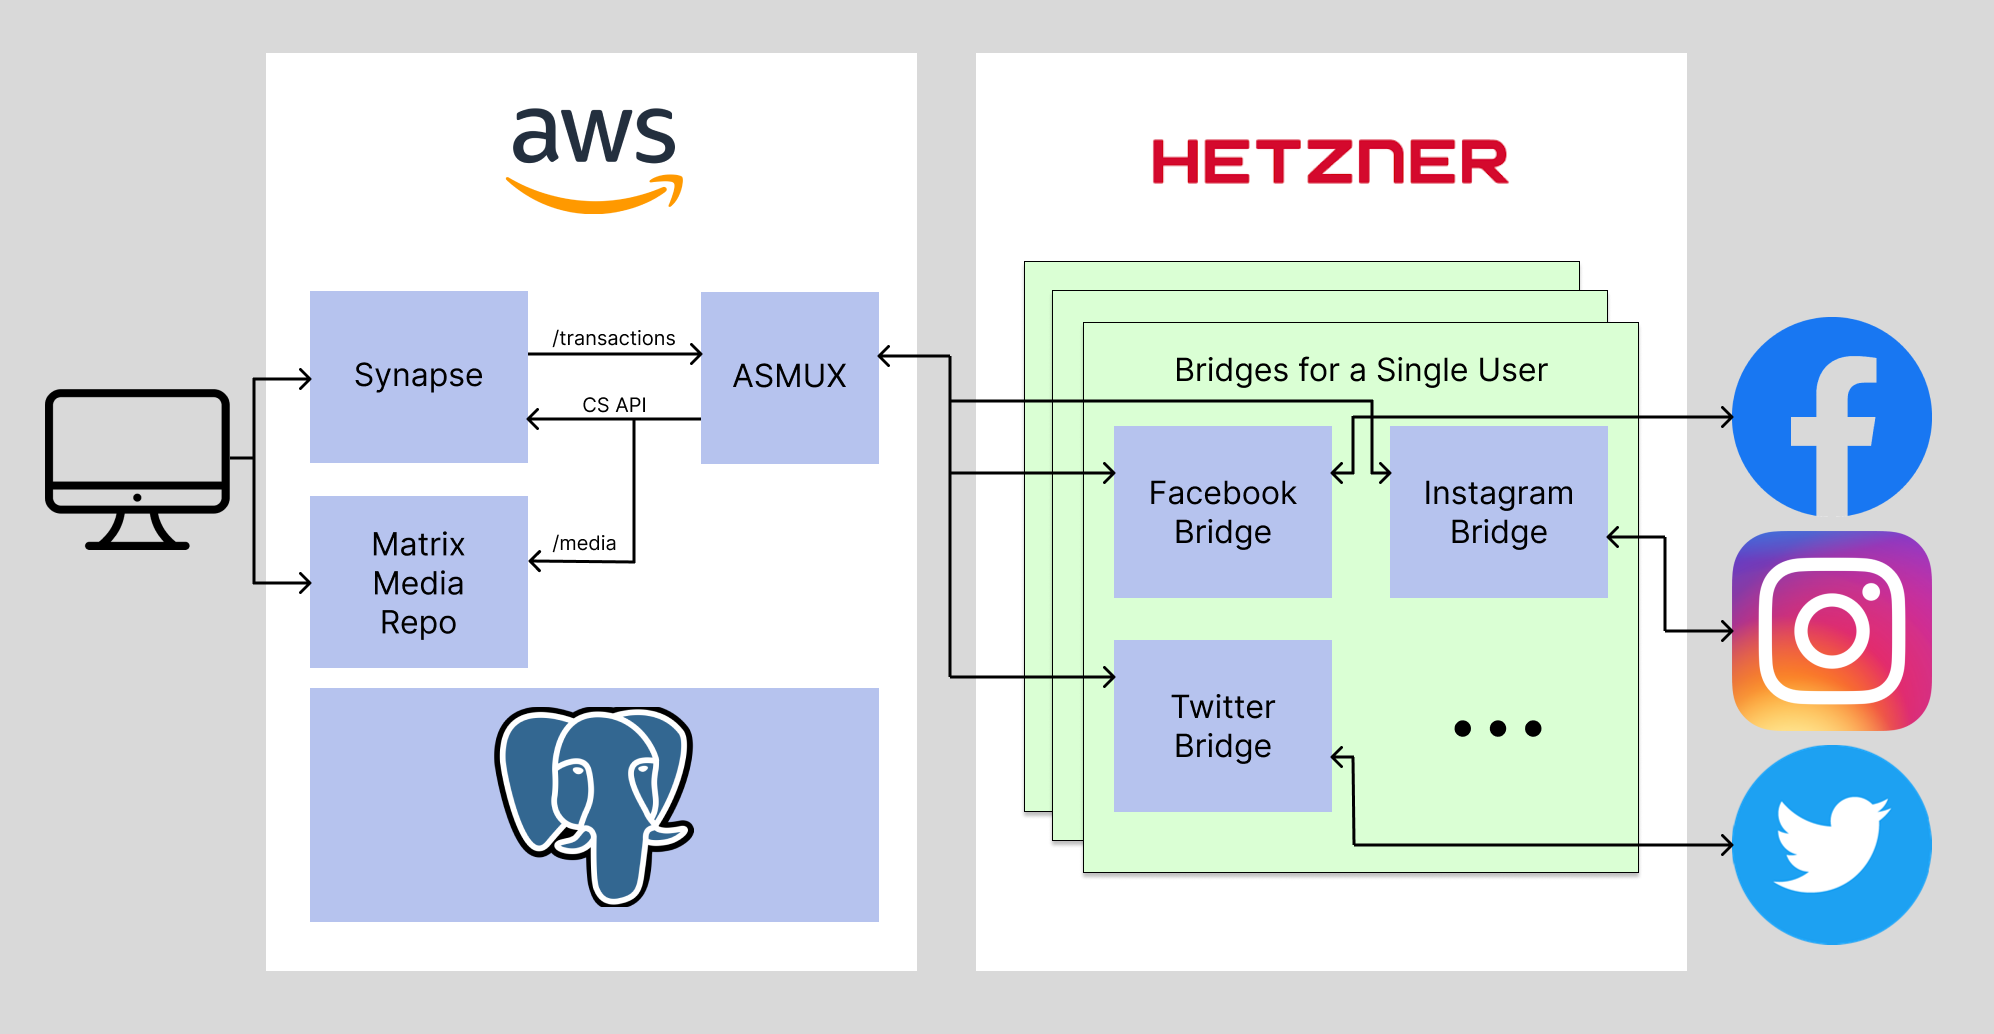
\includegraphics[width=1.15\textwidth]{images/current-architecture}}

    Each user gets their own bridge for each network they connect.
\end{frame}

\begin{frame}{Advantages of our architecture}
    \begin{itemize}[<+->]
        \item Each users' bridge is \textbf{isolated}
        \item We can deploy \textbf{different bridge versions} to different sets
            of users
        \item Bridges can be stopped and started individually
        \item Double puppeting
    \end{itemize}
\end{frame}

\begin{frame}{Disadvantages of our architecture}
    \begin{itemize}[<+->]
        \item We have to run a \textbf{lot} of bridges
        \item Synapse is not designed for a dynamic numbers of bridges
        \item If two users join the same chat on an external network, we end up
            with two rooms with the same data
        \item We run Synapse on AWS which is relatively expensive
        \item Synapse becomes a bottleneck for all traffic
    \end{itemize}
\end{frame}

\begin{frame}{Back to the diagram}
    \centerline{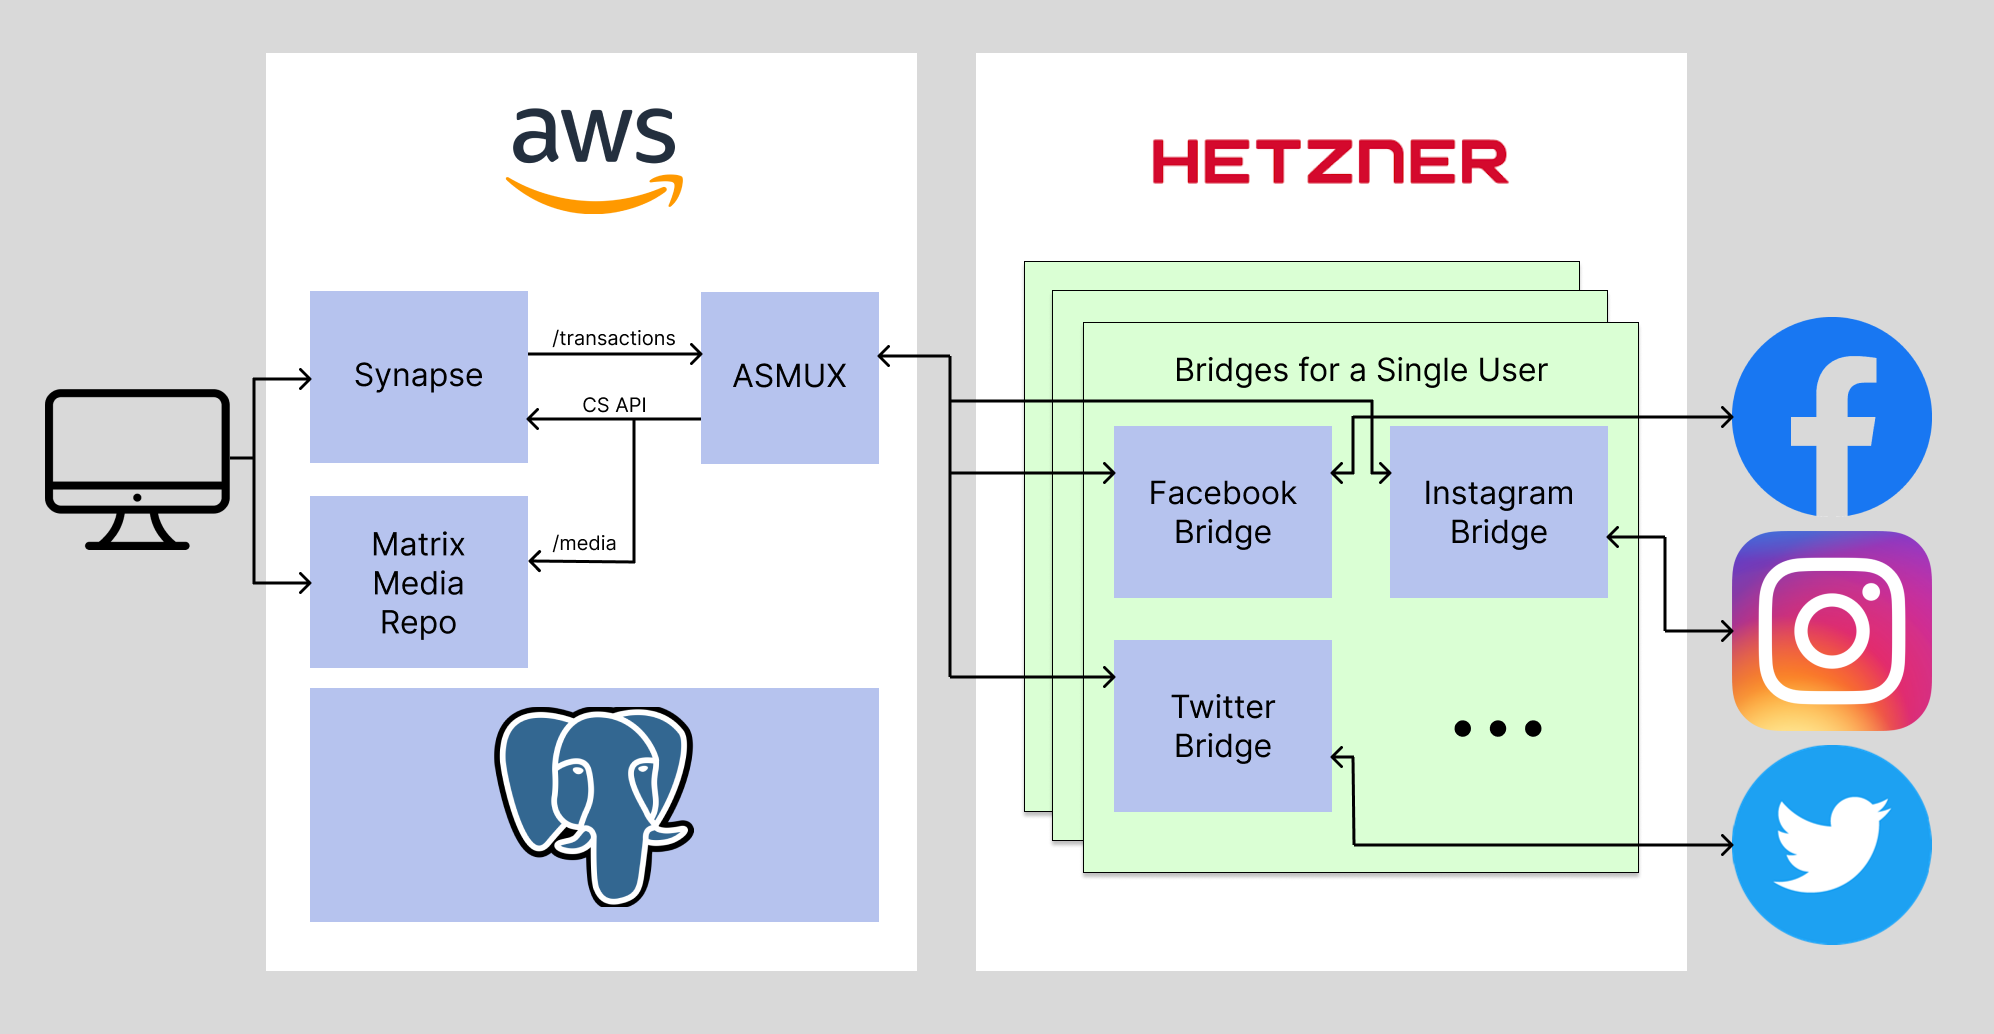
\includegraphics[width=1.15\textwidth]{images/current-architecture}}
    The core software in this architecture is Synapse.
\end{frame}

\begin{frame}{Stats}
    % TODO: stats about the number of puppets per actual user

    None of that traffic is federated, but it has to go to Synapse which is
    designed with federation front-and-center!
\end{frame}

\begin{frame}{A few more notes}
    \begin{itemize}[<+->]
        \item \textbf{Synapse is aggressively federated}

            Synapse has no special handling of federated vs unfederated rooms.

        \item \textbf{Synapse does not handle message floods well}

            Synapse falls over when users bridge some large Telegram chats and
            Discord servers.

        \item \textbf{Deleting rooms from Synapse is hard}

            We end up with lots of \textit{dead} rooms when users delete their
            bridges and never turn it back on (or need a hard bridge reset).
    \end{itemize}
\end{frame}

\begin{frame}[standout]
    \Large
    Solution: build a homeserver optimized for unfederated bridge traffic
\end{frame}

\section{Hungryserv}

\begin{frame}{Why is it hungry?}
    \Large
    Because it's unfed\pause{erated!}
\end{frame}

\begin{frame}{Our new architecture}
    \centerline{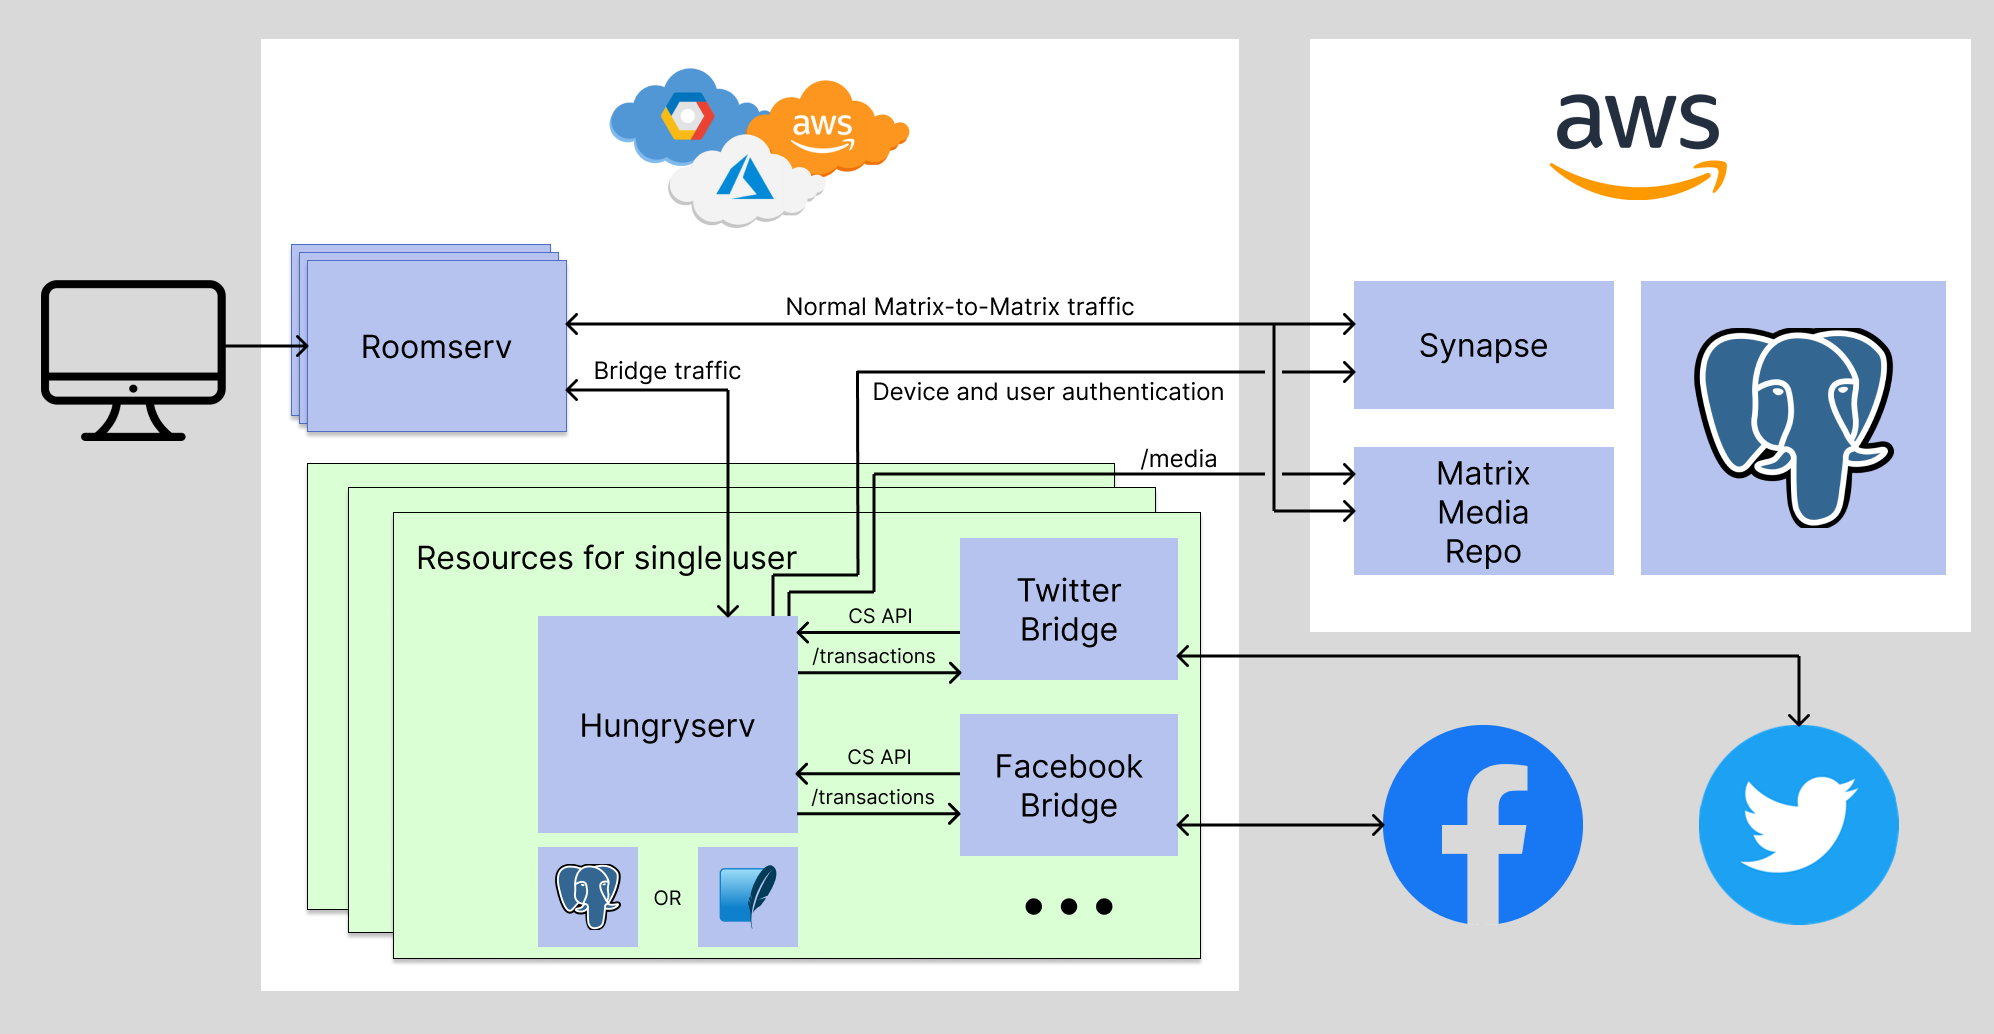
\includegraphics[width=1.15\textwidth]{images/new-architecture}}
\end{frame}

\begin{frame}{Why unfederated?}
    Each bridge belongs to a single user, so federation is unnecessary. \\
    \pause

    \begin{quote}
        When your DAG is a linked-list, don't store it as a DAG.
    \end{quote}
    \pause

    Being unfederated means that we can avoid implementing many of the event
    auth rules.
    \begin{itemize}
        \item Event storage requires less metadata
        \item Deletions can be optimized
        \item Infinite backfill becomes an simple batch SQL operation
    \end{itemize}
\end{frame}

\begin{frame}[standout]
    \Large
    Demo!
\end{frame}

\end{document}
% Local Variables:
% TeX-command-extra-options: "-shell-escape"
% End:
